\documentclass{standalone}
\usepackage{tikz}
\usetikzlibrary{patterns, positioning}


\begin{document}
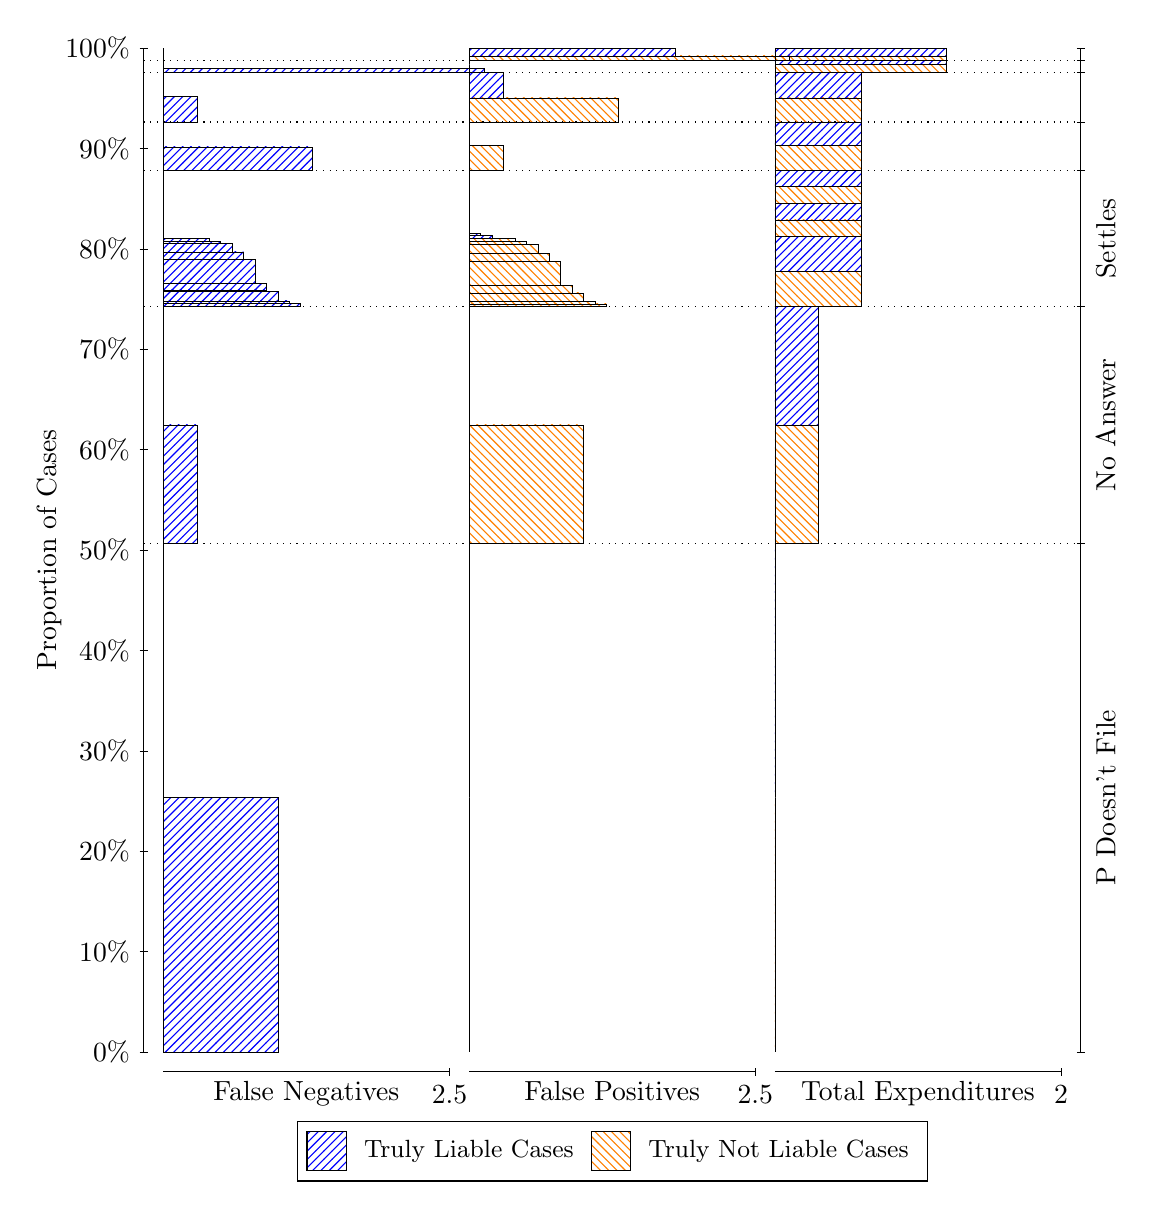
\begin{tikzpicture}
\draw[black, very thin] (1.5,1.75) -- (1.5,14.5);
\node[rotate=90, text=black, anchor=center] at (0.3, 8.125) {Proportion of Cases};
\draw[black, very thin] (1.45,1.75) -- (1.55,1.75);
\node[text=black, anchor=east] at (1.45, 1.75) {0\%};
\draw[black, very thin] (1.45,3.025) -- (1.55,3.025);
\node[text=black, anchor=east] at (1.45, 3.025) {10\%};
\draw[black, very thin] (1.45,4.3) -- (1.55,4.3);
\node[text=black, anchor=east] at (1.45, 4.3) {20\%};
\draw[black, very thin] (1.45,5.575) -- (1.55,5.575);
\node[text=black, anchor=east] at (1.45, 5.575) {30\%};
\draw[black, very thin] (1.45,6.85) -- (1.55,6.85);
\node[text=black, anchor=east] at (1.45, 6.85) {40\%};
\draw[black, very thin] (1.45,8.125) -- (1.55,8.125);
\node[text=black, anchor=east] at (1.45, 8.125) {50\%};
\draw[black, very thin] (1.45,9.4) -- (1.55,9.4);
\node[text=black, anchor=east] at (1.45, 9.4) {60\%};
\draw[black, very thin] (1.45,10.675) -- (1.55,10.675);
\node[text=black, anchor=east] at (1.45, 10.675) {70\%};
\draw[black, very thin] (1.45,11.95) -- (1.55,11.95);
\node[text=black, anchor=east] at (1.45, 11.95) {80\%};
\draw[black, very thin] (1.45,13.225) -- (1.55,13.225);
\node[text=black, anchor=east] at (1.45, 13.225) {90\%};
\draw[black, very thin] (1.45,14.5) -- (1.55,14.5);
\node[text=black, anchor=east] at (1.45, 14.5) {100\%};

\draw[black, very thin] (13.4,1.75) -- (13.4,14.5);
\draw[black, very thin] (13.35,1.75) -- (13.45,1.75);
\node[anchor=west] at (13.35, 1.75) {};
\draw[black, very thin] (13.35,8.2106) -- (13.45,8.2106);
\node[anchor=west] at (13.35, 8.2106) {};
\draw[black, very thin] (13.35,11.216) -- (13.45,11.216);
\node[anchor=west] at (13.35, 11.216) {};
\draw[black, very thin] (13.35,12.949) -- (13.45,12.949);
\node[anchor=west] at (13.35, 12.949) {};
\draw[black, very thin] (13.35,13.561) -- (13.45,13.561);
\node[anchor=west] at (13.35, 13.561) {};
\draw[black, very thin] (13.35,14.19) -- (13.45,14.19);
\node[anchor=west] at (13.35, 14.19) {};
\draw[black, very thin] (13.35,14.345) -- (13.45,14.345);
\node[anchor=west] at (13.35, 14.345) {};
\draw[black, very thin] (13.35,14.5) -- (13.45,14.5);
\node[anchor=west] at (13.35, 14.5) {};

\draw[black, very thin, pattern color=blue, pattern=north east lines] (1.75,1.75) rectangle (3.2033,4.9803);
\draw[black, very thin, pattern color=orange, pattern=north west lines] (1.75,4.9803) rectangle (1.75,8.2106);
\draw[black, very thin, pattern color=blue, pattern=north east lines] (1.75,8.2106) rectangle (2.186,9.7135);
\draw[black, very thin, pattern color=orange, pattern=north west lines] (1.75,9.7135) rectangle (1.75,11.216);
\draw[black, very thin, pattern color=blue, pattern=north east lines] (1.75,11.216) rectangle (3.494,11.254);
\draw[black, very thin, pattern color=blue, pattern=north east lines] (1.75,11.254) rectangle (3.3487,11.288);
\draw[black, very thin, pattern color=blue, pattern=north east lines] (1.75,11.288) rectangle (3.2033,11.405);
\draw[black, very thin, pattern color=blue, pattern=north east lines] (1.75,11.405) rectangle (3.058,11.427);
\draw[black, very thin, pattern color=blue, pattern=north east lines] (1.75,11.427) rectangle (3.058,11.51);
\draw[black, very thin, pattern color=blue, pattern=north east lines] (1.75,11.51) rectangle (2.9127,11.817);
\draw[black, very thin, pattern color=blue, pattern=north east lines] (1.75,11.817) rectangle (2.7673,11.91);
\draw[black, very thin, pattern color=blue, pattern=north east lines] (1.75,11.91) rectangle (2.622,12.015);
\draw[black, very thin, pattern color=blue, pattern=north east lines] (1.75,12.015) rectangle (2.4767,12.049);
\draw[black, very thin, pattern color=blue, pattern=north east lines] (1.75,12.049) rectangle (2.3313,12.084);
\draw[black, very thin, pattern color=orange, pattern=north west lines] (1.75,12.084) rectangle (1.75,12.949);
\draw[black, very thin, pattern color=blue, pattern=north east lines] (1.75,12.949) rectangle (3.6393,13.244);
\draw[black, very thin, pattern color=orange, pattern=north west lines] (1.75,13.244) rectangle (1.75,13.561);
\draw[black, very thin, pattern color=blue, pattern=north east lines] (1.75,13.561) rectangle (2.186,13.885);
\draw[black, very thin, pattern color=orange, pattern=north west lines] (1.75,13.885) rectangle (1.75,14.19);
\draw[black, very thin, pattern color=blue, pattern=north east lines] (1.75,14.19) rectangle (5.8193,14.246);
\draw[black, very thin, pattern color=orange, pattern=north west lines] (1.75,14.246) rectangle (1.75,14.345);
\draw[black, very thin, pattern color=orange, pattern=north west lines] (1.75,14.345) rectangle (1.75,14.401);
\draw[black, very thin, pattern color=blue, pattern=north east lines] (1.75,14.401) rectangle (1.75,14.5);
\draw[black, very thin, pattern color=orange, pattern=north west lines] (5.6333,1.75) rectangle (5.6333,4.9803);
\draw[black, very thin, pattern color=blue, pattern=north east lines] (5.6333,4.9803) rectangle (5.6333,8.2106);
\draw[black, very thin, pattern color=orange, pattern=north west lines] (5.6333,8.2106) rectangle (7.0867,9.7135);
\draw[black, very thin, pattern color=blue, pattern=north east lines] (5.6333,9.7135) rectangle (5.6333,11.216);
\draw[black, very thin, pattern color=orange, pattern=north west lines] (5.6333,11.216) rectangle (7.3773,11.251);
\draw[black, very thin, pattern color=orange, pattern=north west lines] (5.6333,11.251) rectangle (7.232,11.282);
\draw[black, very thin, pattern color=orange, pattern=north west lines] (5.6333,11.282) rectangle (7.0867,11.389);
\draw[black, very thin, pattern color=orange, pattern=north west lines] (5.6333,11.389) rectangle (6.9413,11.486);
\draw[black, very thin, pattern color=orange, pattern=north west lines] (5.6333,11.486) rectangle (6.796,11.792);
\draw[black, very thin, pattern color=orange, pattern=north west lines] (5.6333,11.792) rectangle (6.6507,11.893);
\draw[black, very thin, pattern color=orange, pattern=north west lines] (5.6333,11.893) rectangle (6.5053,12.007);
\draw[black, very thin, pattern color=orange, pattern=north west lines] (5.6333,12.007) rectangle (6.36,12.043);
\draw[black, very thin, pattern color=orange, pattern=north west lines] (5.6333,12.043) rectangle (6.2147,12.082);
\draw[black, very thin, pattern color=blue, pattern=north east lines] (5.6333,12.082) rectangle (5.924,12.116);
\draw[black, very thin, pattern color=blue, pattern=north east lines] (5.6333,12.116) rectangle (5.7787,12.15);
\draw[black, very thin, pattern color=blue, pattern=north east lines] (5.6333,12.15) rectangle (5.6333,12.949);
\draw[black, very thin, pattern color=orange, pattern=north west lines] (5.6333,12.949) rectangle (6.0693,13.265);
\draw[black, very thin, pattern color=blue, pattern=north east lines] (5.6333,13.265) rectangle (5.6333,13.561);
\draw[black, very thin, pattern color=orange, pattern=north west lines] (5.6333,13.561) rectangle (7.5227,13.866);
\draw[black, very thin, pattern color=blue, pattern=north east lines] (5.6333,13.866) rectangle (6.0693,14.19);
\draw[black, very thin, pattern color=orange, pattern=north west lines] (5.6333,14.19) rectangle (5.6333,14.289);
\draw[black, very thin, pattern color=blue, pattern=north east lines] (5.6333,14.289) rectangle (5.6333,14.345);
\draw[black, very thin, pattern color=orange, pattern=north west lines] (5.6333,14.345) rectangle (9.7027,14.401);
\draw[black, very thin, pattern color=blue, pattern=north east lines] (5.6333,14.401) rectangle (8.2493,14.5);
\draw[black, very thin, pattern color=orange, pattern=north west lines] (9.5167,1.75) rectangle (9.5167,4.9803);
\draw[black, very thin, pattern color=blue, pattern=north east lines] (9.5167,4.9803) rectangle (9.5167,8.2106);
\draw[black, very thin, pattern color=orange, pattern=north west lines] (9.5167,8.2106) rectangle (10.062,9.7135);
\draw[black, very thin, pattern color=blue, pattern=north east lines] (9.5167,9.7135) rectangle (10.062,11.216);
\draw[black, very thin, pattern color=orange, pattern=north west lines] (9.5167,11.216) rectangle (10.607,11.661);
\draw[black, very thin, pattern color=blue, pattern=north east lines] (9.5167,11.661) rectangle (10.607,12.106);
\draw[black, very thin, pattern color=orange, pattern=north west lines] (9.5167,12.106) rectangle (10.607,12.317);
\draw[black, very thin, pattern color=blue, pattern=north east lines] (9.5167,12.317) rectangle (10.607,12.528);
\draw[black, very thin, pattern color=orange, pattern=north west lines] (9.5167,12.528) rectangle (10.607,12.738);
\draw[black, very thin, pattern color=blue, pattern=north east lines] (9.5167,12.738) rectangle (10.607,12.949);
\draw[black, very thin, pattern color=orange, pattern=north west lines] (9.5167,12.949) rectangle (10.607,13.265);
\draw[black, very thin, pattern color=blue, pattern=north east lines] (9.5167,13.265) rectangle (10.607,13.561);
\draw[black, very thin, pattern color=orange, pattern=north west lines] (9.5167,13.561) rectangle (10.607,13.866);
\draw[black, very thin, pattern color=blue, pattern=north east lines] (9.5167,13.866) rectangle (10.607,14.19);
\draw[black, very thin, pattern color=orange, pattern=north west lines] (9.5167,14.19) rectangle (11.697,14.289);
\draw[black, very thin, pattern color=blue, pattern=north east lines] (9.5167,14.289) rectangle (11.697,14.345);
\draw[black, very thin, pattern color=orange, pattern=north west lines] (9.5167,14.345) rectangle (11.697,14.401);
\draw[black, very thin, pattern color=blue, pattern=north east lines] (9.5167,14.401) rectangle (11.697,14.5);
\draw[black, dotted] (1.5,8.2106) -- (13.4,8.2106);
\draw[black, dotted] (1.5,11.216) -- (13.4,11.216);
\draw[black, dotted] (1.5,12.949) -- (13.4,12.949);
\draw[black, dotted] (1.5,13.561) -- (13.4,13.561);
\draw[black, dotted] (1.5,14.19) -- (13.4,14.19);
\draw[black, dotted] (1.5,14.345) -- (13.4,14.345);
\draw[black, very thin] (1.75,1.5) -- (5.3833,1.5);
\node[text=black, anchor=north] at (3.5667, 1.5) {False Negatives};
\draw[black, very thin] (5.3833,1.45) -- (5.3833,1.55);
\node[text=black, anchor=north] at (5.3833, 1.45) {2.5};

\draw[black, very thin] (5.6333,1.5) -- (9.2667,1.5);
\node[text=black, anchor=north] at (7.45, 1.5) {False Positives};
\draw[black, very thin] (9.2667,1.45) -- (9.2667,1.55);
\node[text=black, anchor=north] at (9.2667, 1.45) {2.5};

\draw[black, very thin] (9.5167,1.5) -- (13.15,1.5);
\node[text=black, anchor=north] at (11.333, 1.5) {Total Expenditures};
\draw[black, very thin] (13.15,1.45) -- (13.15,1.55);
\node[text=black, anchor=north] at (13.15, 1.45) {2};

\node[text=black, centered, rotate=90] at (13.72, 4.9803) {P Doesn't File};
\node[text=black, centered, rotate=90] at (13.72, 9.7135) {No Answer};
\node[text=black, centered, rotate=90] at (13.72, 12.083) {Settles};





\draw (7.449999999999999,1.5) node[draw=none] (baseCoordinate) {};
\begin{scope}[align=center]
        \matrix[scale=0.5, draw=black, below=0.5cm of baseCoordinate, nodes={draw}, column sep=0.1cm]{
            \node[rectangle, draw, minimum width=0.5cm, minimum height=0.5cm, pattern color=blue, pattern=north east lines] {}; &
            \node[draw=none, font=\small, text=black] (B) {Truly Liable Cases}; &
            \node[rectangle, draw, minimum width=0.5cm, minimum height=0.5cm, pattern color=orange, pattern=north west lines] {}; &
            \node[draw=none, font=\small, text=black] (B) {Truly Not Liable Cases}; \\
            };
\end{scope}

\end{tikzpicture}
\end{document}